\documentclass{beamer}
\usepackage{listings}
\usepackage{booktabs}
\usepackage{bookmark}
\usepackage{makecell}
\usepackage{url}
\usepackage{multirow}
\usepackage{graphicx}
\usepackage[spanish]{babel}
\usepackage{beamerthemesplit}
\usetheme{Warsaw}

\lstdefinestyle{latexStyle}{
    language=[LaTeX]{TeX},
    belowcaptionskip=1\baselineskip,
    breaklines=true,
    frame=none,
    numbers=none, 
    basicstyle=\footnotesize\ttfamily,
    keywordstyle=\bfseries\color{green!40!black},
    commentstyle=\itshape\color{purple!40!black},
    identifierstyle=\color{blue},
    backgroundcolor=\color{blue!10!white},
}
\lstset{style=latexStyle}

\title{Proyecto Moogle}
\subtitle{}
\institute{Facultad de Matemática y Computación\\Universidad de la Habana}
\author{Abraham Romero Imbert}
\date{Julio, 2023}

\begin{document}
\maketitle

\begin{frame}
  \frametitle{Contenido}
  \begin{enumerate}
    \item \Huge\textbf{¿Qué es Moogle?}
    \item  \Huge\textbf{¿Cómo funciona?}
  \end{enumerate}
\end{frame}

\begin{frame}
  \frametitle{ Introducción}
\begin{center}
  \LARGE\textbf{¿Qué es Moogle?}
\end{center}
\begin{figure}[h]
    \center
    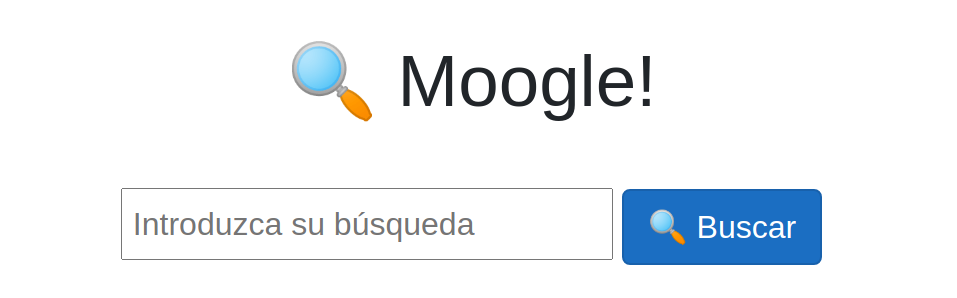
\includegraphics[width=8cm]{moogle.png}
    \caption{Imagen de Moogle!}
    \label{fig:Moogle}
\end{figure}
Es el primer proyecto de Programación orientado a Primer Año de Ciencias de la Computación.
Básicamente es una aplicación cuyo propósito es buscar inteligentemente un texto en un conjunto de documentos.
\end{frame}

\begin{frame}
\frametitle{Funcionamiento}
\begin{center}
  \LARGE\textbf{¿Cómo funciona?}
\end{center}
Como cualquier buscador busca información en una base de datos a partir de palabras clave o frases que el usuario introduce en la barra de búsqueda.  
Utiliza algoritmos para encontrar archivos que contienen las palabras clave y las presenta al usuario en una lista de resultados teniendo en cuenta la relevancia de los mismos respecto a la búsqueda realizada
Adicionalmente este buscador tiene la capacidad de sugerir al usuario otras posibles  búsquedas, en especial al no encontrar resultados en la base de datos
\end{frame}

\begin{frame}
\frametitle{Algoritmo del Programa}
\framesubtitle{Explicación básica del funcionamiento}
Debido a que el algoritmo utilizado en mi proyecto es explicado más detalladamente en un informe dentro del mismo proyecto en esta presentación solo se eplicará de manera superficial
\end{frame}

\begin{frame}
\frametitle{Algoritmo del Programa}
\framesubtitle{Explicación básica del funcionamiento}
El programa se ejecuta dentro de la clase Moogle y desde la ubicación del programa en la computadora
Luego va a la carpeta Content(donde se encuentran los archivos o base de datos entre los cuales se darán los resultados) y analiza cada uno de los documentos para generar un objeto de la clase DiccionarioReferencial el cual almacena los datos necesarios para efectuar el cálculo de la relación TF-IDF (mide la relevancia de una palabra o parte de un documento con el query del usuario)
\end{frame}

\begin{frame}
\frametitle{Algoritmo del Programa}
\framesubtitle{Explicación básica del funcionamiento}
Luego se genera otro objeto estático de la clase MatrizTFIDF que es la representación en valores de TF-IDF de cada documento y término de la base de datos
Este objeto es en sí un array de objetos ¨Vector¨. Cada uno de estos vectores n-dimensionales(n definido por la cantidad de términos diferentes) están representados por valores double definidos por la relevancia(o repetición) de cada término en el documento y en el espacio de la base de datos.
El cálculo de TF-IDF se efectúa con la siguiente fórmula:
\end{frame}

\begin{frame}
\frametitle{Algoritmo del Programa}
\framesubtitle{Explicación básica del funcionamiento}
\begin{equation}\label{eq:TF*IDF}
TF\cdot IDF
\end{equation}

Donde 

\begin{equation}\label{eq:TF}
TF_{i}=\frac{\log_{2}(Freq(i,j)+1)}{\log_{2}(L_{j}+0.001)}
\end{equation}

Freq(i,j)+1 = Frecuencia del término i en el documento j.

$L_{j}$ = Número total de términos en el documento j. En este caso se le sumo a este valor 0.001 para evitar indefiniciones en la función 

\begin{equation}\label{eq:IDF}
IDF_{i} = log_{2}(1+\frac{N_{d}}{f_{i}+1})
\end{equation}
$N_{d}$ = Número total de documentos considerados\\
$f_{i}$ = Número de documentos que contienen el término i. En este caso se le sumo a este valor 1 para evitar indefiniciones en la función 
\end{frame}

\begin{frame}
\frametitle{Algoritmo del Programa}
\framesubtitle{Explicación básica del funcionamiento}
Una vez el usuario ha ingresado el query(o cunsulta) la clase Query-class se encarga de analizar dicha entrada y procesarla para después compararla con cada documento y devolver los resultados. Esto se hace mediante la fórmula siguiente que mide la similitud de dos vectores en un espacio n-dimensional:
\begin{equation}
\cos(\theta) = \frac{A\cdot B}{\parallel A\parallel \* \parallel B\parallel}= \frac{\sum\limits_{i=1}^n A_i\* B_i}{\sqrt{\sum\limits_{i=1}^n A_i^2}\* \sqrt{\sum\limits_{i=1}^n B_i^2}}
\end{equation}
\end{frame}

\begin{frame}
\frametitle{Algoritmo del Programa}
\framesubtitle{Explicación básica del funcionamiento}
Dentro de esta misma clase también se elabora un Snippet (o un fragmento del documento donde aparece su parte más parecida al query del usuario), así como una sugerencia de query válido lo más parecido posible al del usuario. Ejemplo:
\begin{figure}[h]
    \center
    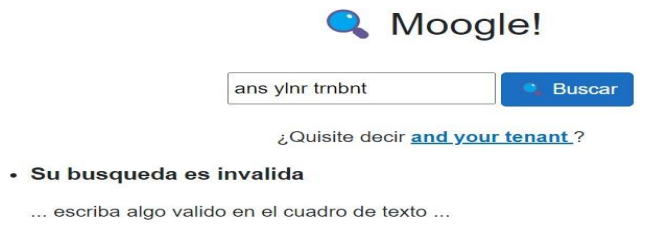
\includegraphics[width=8cm]{suggestion.png}
    \caption{Sugerencia en Moogle!}
    \label{fig:suggestion}
\end{figure}
\end{frame}

\begin{frame}
  \frametitle{Resumen}
  De esta manera se ha explicado brevemente el funcionamiento o implementación de mi proyecto Moogle!.Este puede estar sujeto a cambios más adelante que le brinden más funcionaliad o eficiencia. Tenga en cuenta que dentro del mismo proyecto se encuentra un informe que explica más detalladamente cada proceso de ejecución del programa.
\end{frame}
\maketitle
\begin{frame}
\center
\Huge\textbf{Muchas Gracias}
\end{frame}





















\end{document}
